\section{Results}
\label{results}

\subsection{Sentiment Analysis}
Given the abundance of UNSC session data available, we decided to narrow the scope of our analysis using different approaches. First, we examined to most popular topics in order the determine whether trends can be seen. Secondly, we took a look at the big picture and analyzed the sentiment development for each country in the time frame 1995-2017. Finally, we decided to analyze the core nations of the UNSC, since the corpus provides consistent data for the entire time frame. In addition to this, we analyzed the sentiment in Iraq War related sessions. 
\subsubsection{Topics}
In order to get a grasp of the contents of the sessions, we examined the most common topics for the provided time frame and each year respectively. Figure \ref{common_1} visualizes the 20 most common topics for the UNSC speeches. It can be observed that there is no uniform naming convention for the topics. The most discussed topic is \textit{Middle East situation, including the Palestinian question} and the topic on rank six is \textit{The situation in the Middle East, including the Palestinian question}. In other analyses, the topic name \textit{The situation in the Middle East} occurs as well. It can be assumed that the different topic names refer to one and the same topic.  
Interestingly, the Middle East topic occurs in the most discussed topics for the first time in 2000 and remains in the top 5 most discussed topics for the entirety of 2000-2017, despite the inconsistent naming convention.

\begin{figure}[t]
  \centering
  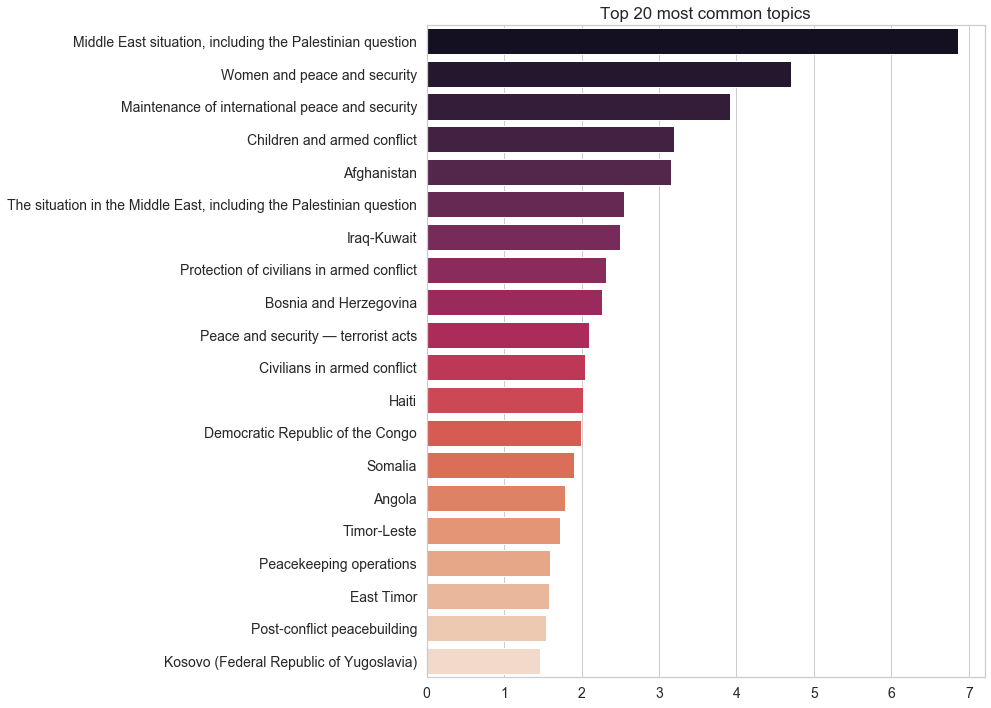
\includegraphics[width=14.5cm]{img/20most_common_topics.png}
  \caption{The 20 most common topics in the UNSC}
  \label{common_1}
\end{figure}%

A shift in topics can be observed after the year 2001. The most common topics diverged from humanitarian ones (e.g. Africa, Angola, East Timor) to more fundamental ones (e.g. Peace and Security - terrorist acts, Women and Peace and Security, Post-conflict peacebuilding). Figure \ref{common_2} and Figure \ref{common_3} visualize the differences in topics for 1996 and 2003. 
\begin{figure}[t]
  \centering
  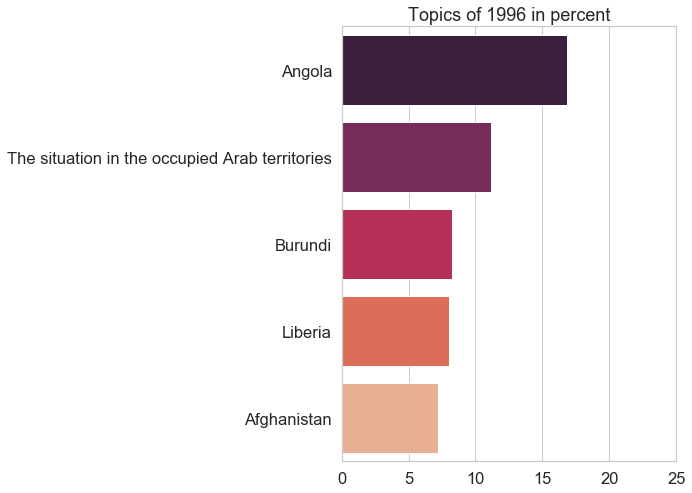
\includegraphics[width=13cm]{img/1996_most_common_topics.png}
  \caption{Most common topics in 1996}
  \label{common_2}
\end{figure}%

\subsubsection{Sentiment in the UNSC}
The sentiment analysis in the UNSC was conducted on 182 individual members of the council, sovereign nations and independent members were included. As could be expected, the participation varies among the members. For some countries, only scarce data is available, e.g. Belize, which only took part in four years of council meetings. Other countries attended the council meetings more frequently, with many countries appearing in all 23 years of the analysis. It is also worth noting that some countries' names changed over time, e.g. Zaire, which is now known as Democratic Republic of the Congo, and some countries do not exist anymore, e.g. the former Yugoslavia.

\begin{figure}[t]
  \centering
  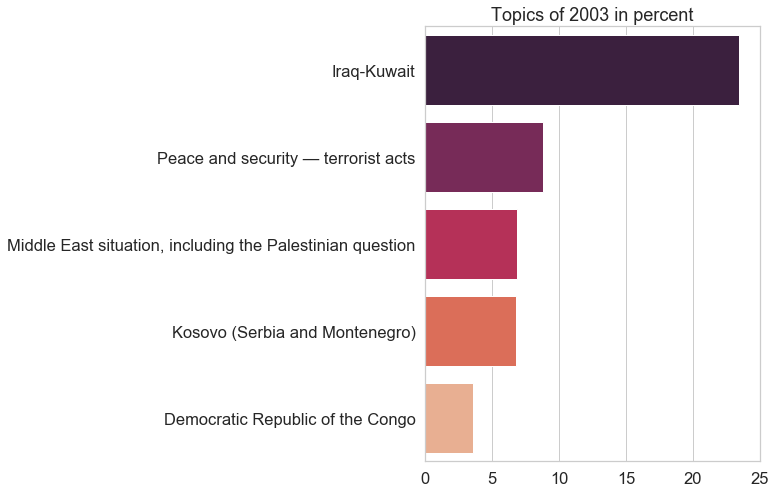
\includegraphics[width=13cm]{img/2003_most_common_topics.png}
  \caption{Most common topics in 2003}
  \label{common_3}
    \centering
    \vspace{10pt}
    \begin{minipage}{0.47\textwidth}
        \centering
        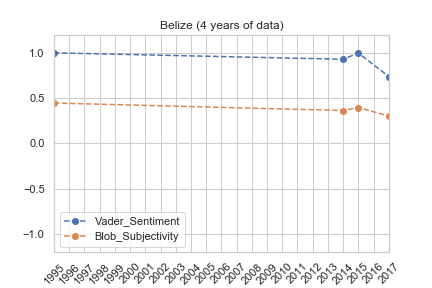
\includegraphics[width=1.1\textwidth]{img/Belize_average.png} % first figure itself
        \caption{Sentiment Analysis for Belize}
        \label{belize}
    \end{minipage}\hfill
    \begin{minipage}{0.47\textwidth}
        \centering
        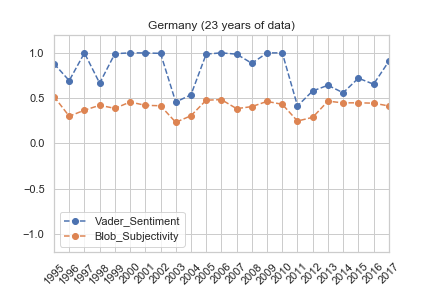
\includegraphics[width=1.1\textwidth]{img/Germany_average.png} % second figure itself
        \caption{Sentiment Analysis for Germany}
        \label{germany}
    \end{minipage}
\end{figure}

The visualizations of the sentiment and subjectivity analysis for Belize (Figure \ref{belize}) and Germany (Figure \ref{germany}) suggest a correlation between sentiment and subjectivity scores. A higher polarity in sentiment occurs with an increase in subjectivity in the analysis for Belize, while the lower sentiment scores come with an increase in objectivity for Germany. For Germany, especially the year 2003 stands out. 2003 was the beginning of the Iraq War, of which Germany was a vocal opponent \citep{germiraq}.

\subsubsection{Sentiment in the Core Nations}
After completing the topic and sentiment analysis for the UNSC, we decided to narrow the scope of our investigations. A comparative and exploratory analysis yields the best results if the data is not skewed, i.e. equally distributed. For this reason, we laid our focus for the sentiment analysis on the core nations of the UNSC, which are the People's Republic of China, the French Republic, the Russian Federation, the United Kingdom of Great Britain and Northern Ireland, and the United States of America.

These core nation are granted a permanent member status of the council as per the Charter of the United Nations, a treaty from 1945\footnote{\href{https://www.un.org/en/charter-united-nations/}{https://www.un.org/en/charter-united-nations/}}. A permanent membership entails a \textit{Power of Veto}, which allows voting against UNSC resolutions and thus preventing their adoption. 
The core nations were a suitable subject for our analysis since they participated in most of the UNSC meetings. Not only could we rely on data for every year provided in the corpus, we could also assume that important resolutions would be included in the analysis.

\begin{figure}[t]
  \centering
  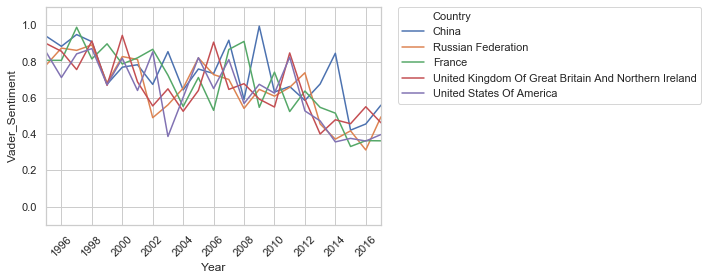
\includegraphics[width=14.75cm]{img/over_time_Vader_Sentiment.png}
  \caption{Sentiment development in the UNSC core nations}
  \label{fig:vadercore}
\end{figure}%

\begin{figure}[t]
  \centering
  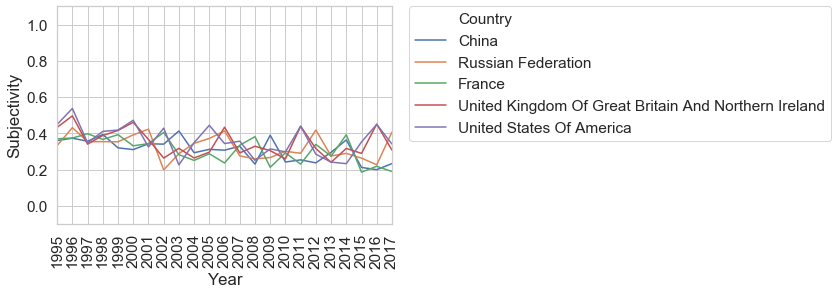
\includegraphics[width=14.75cm]{img/over_time_Blob_Subjectivityy.png}
  \caption{Subjectivity development in the UNSC core nations}
  \label{fig:subjcore}
\end{figure}%

The sentiment analysis for the UNSC core nations shows a general downward trend in sentiment polarity (Figure \ref{fig:vadercore}). Significant negative peaks were revealed for historical events, e.g. the year 2002 for the Russian Federation and the year 2003 for the United States of America, both possibly related to the imminent Iraq War.

The visualization of the subjectivity analysis (Figure  \ref{fig:subjcore}) shows a mostly consistent development of subjectivity in the core nations but suggests a slight downward trend, meaning a rise in objectivity, over the investigated time frame. This is consistent with the observation made in %link subsubsection sentiment in the unsc 
the sentiment analysis conducted on all members of the UNSC. The negative peaks in sentiment mentioned for Russia and the USA, 2002 and 2003 respectively, also appear as negative, more objective, peaks in the subjectivity analysis.

\subsubsection{Sentiment regarding the Iraq War}
%%% should this go in background info??
As the topic for an in-depth analysis, we chose the Iraq War. Until today, the Iraq War and the UNSC's involvement in it is a highly polarizing topic. Kofi Annan, the United Nations Secretary-General, stated that ``the US-led invasion of Iraq was an illegal act that contravened the UN charter" \citep{bbciraq}.
The possibility of an invasion arose from the speculation that Iraq was in possession of weapons of mass destruction, after the UNSC council unanimously adopted Resolution 1441 which gave Iraq "a final opportunity to comply with its disarmament obligations" \citep{resolution1441}.
This issue also divided the core nations of the Security Council.

The United States of America were a strong proponent of pursuing military action against Iraq, with or without approval of the UNSC \citep{usairaq}. The United Kingdom supported this policy.
France on the other hand was strictly against the war. The former president Jacques Chirac went as far as saying he would make use of his veto right to prevent the adoption of a resolution that would allow for a military intervention in Iraq \citep{nyt}.
China was more reserved in taking a position on this matter, yet stated that their position was ``extremely close to that of France" \citep{cnn}. Russia also did not have a consistent policy on this matter, first being against an invasion and later on becoming more neutral and even approving of the USA's plans \citep{russiairaq}.
On March 19, 2003, an U.S.-led coalition invaded Iraq.

\vspace{-5pt}
\paragraph{General Sentiment}
In order to examine the general sentiment of the core nations regarding the Iraq War, we extracted all speeches with a topic labelled ``Iraq" or ``Iraq-Kuwait". 

\begin{figure}[t!]
    \centering
    \begin{minipage}{0.47\textwidth}
        \centering
        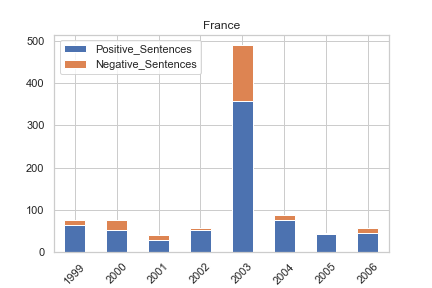
\includegraphics[width=1.1\textwidth]{iraq_scores_France.png} % first figure itself
        \caption{Polarity distribution regarding \\ Iraq for France}
        \label{iraqfr}
    \end{minipage}\hfill
    \begin{minipage}{0.47\textwidth}
        \centering
        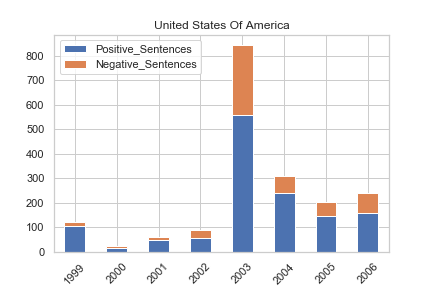
\includegraphics[width=1.1\textwidth]{iraq_scores_United States Of America.png} % second figure itself
        \caption{Polarity distribution regarding \\ Iraq for the USA}
        \label{iraqusa}
    \end{minipage}
\end{figure}

\begin{figure}[t!]
    \centering
    \begin{minipage}{0.47\textwidth}
        \centering
        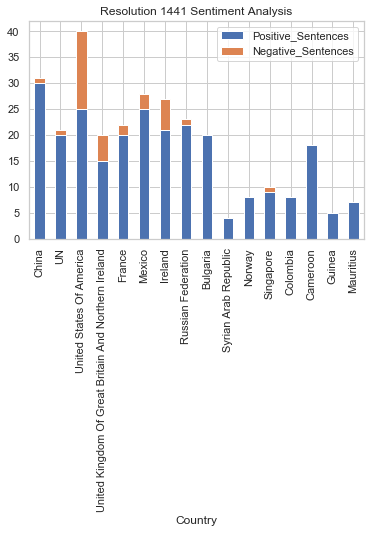
\includegraphics[height=1.7\textwidth]{Resolution 1441_sentiment.png} % first figure itself
        \caption{Sentiment regarding Resolution \\ 1441}
        \label{1441sent}
    \end{minipage}\hfill
    \begin{minipage}{0.47\textwidth}
        \centering
        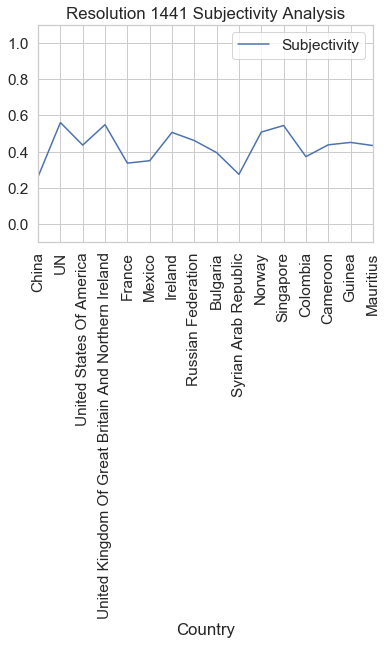
\includegraphics[height=1.7\textwidth]{Resolution 1441_subjectivity.png} % second figure itself
        \caption{Subjectivity regarding Resolution \\ 1441}
        \label{1441subj}
    \end{minipage}
\end{figure}

For presenting the results of the analysis, we chose two countries with opposing opinions on the invasion of Iraq, France (Figure \ref{iraqfr}) and the United States of America (Figure \ref{iraqusa}).
For both countries, the amount of sentences with polarity with regard to Iraq is the highest for the year 2003, due to the Iraq War. Before and after 2003, France contributed on average less than 100 sentences on this topic, an increase after 2003 cannot be observed. This is different for the USA. Before 2003, the analysis reveals years were the country contributed fewer sentences than France, with 1999 being the the year with the most contributions and 2000 being the year with the fewest. After 2003, the USA consistently contributed more than 200 negative and positive sentences per year, which is significantly more than all other core nations.

In 2003, the representatives of the USA contributed more than 800 sentences with polarity, with roughly a third of them being negative. 
For France, the country representatives uttered almost 500 relevant sentences with roughly a quarter of them being negative.

\paragraph{In-Depth: Iraq War related Resolutions}
In order to give a better insight into Iraq War related resolutions, we focused on two sessions that were highly significant in the year leading to the invasion of Iraq. First, we examined Resolution 1441, a resolution that was adopted in the 4644th session of the UNSC on 18 November 2002. As mentioned before, it granted Iraq "a final opportunity to comply with its disarmament obligations" \citep{resolution1441} and subsequently lead to the invasion of Iraq, after the country allegedly failed to comply with said disarmament obligations.

\begin{figure}[b!]
    \centering
    \begin{minipage}{0.45\textwidth}
        \centering
        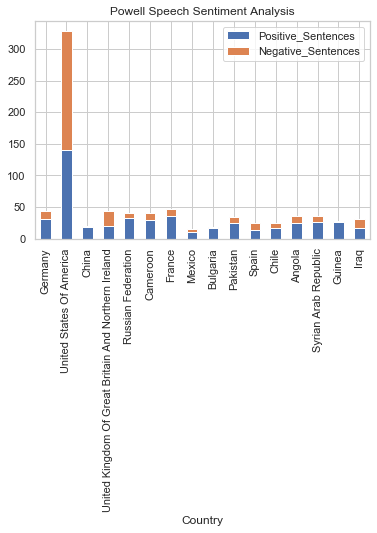
\includegraphics[height=1.7\textwidth]{Powell Speech_sentiment.png} % first figure itself
        \caption{Sentiment regarding Powell's \\ speech}
        \label{powellsent}
    \end{minipage}\hfill
    \begin{minipage}{0.45\textwidth}
        \centering
        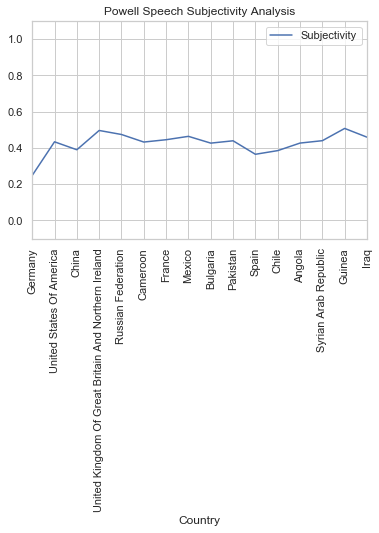
\includegraphics[height=1.7\textwidth]{Powell Speech_subjectivity.png} % second figure itself
        \caption{Subjectivity regarding Powell's \\ speech}
        \label{powellsubj}
    \end{minipage}
\end{figure}

In the sentiment analysis visualizations (Figure \ref{1441sent}) it can be observed that the USA contributed more to the session than the other countries. The highest negative/positive sentence ratio can be observed for the USA and the UK, along with Ireland. While the former two countries were in favor of the ``consequences" announced in Resolution 1441, Ireland had a neutral stance on this policy.

The subjectivity scores (Figure \ref{1441subj}) are roughly distributed between 0.3 and 0.6, which indicates a varying level of objectivity with regard to this resolution.

Secondly, we analyzed session 4701 from February 5, 2003 in which United States Secretary of State Colin Powell discussed the urgency of attacking Iraq as it was allegedly in possession of a mobile production facility for biological weapons \citep{cia}. This speech was controversial in the UNSC and later on it became evident that it was not based on facts but solely on speculations. Neither the USA nor the UK were able to provide evidence for their claims \citep{iraqev}. 
Powell himself said later: ``I regret it. I will always regret it. It was a terrible mistake on all our parts and on the intelligence community." \citep{powell}.

It can be observed that Powell (i.e. the USA) uses a very negative vocabulary (Figure \ref{powellsent}). He contributes significantly more than the other participants (~330 sentences) and more than half of his speech has a negative polarity. A similar ratio of positive to negative sentences can be observed for the UK, although they do not participate more than the other countries involved. This aligns with the previously discussed division of the UNSC regarding the invasion of Iraq and the fact that the USA and the UK were proponents of this approach.

The subjectivity scores (Figure \ref{powellsubj}) concerning the Powell session seem rather homogeneous in comparison to the ones regarding Resolution 1441, except for Germany, which has an unusually low subjectivity score. As discussed before, Germany was a strong opponent of the Iraq War.

\subsection{Argumentation Mining}
\subsubsection{Model Fine-Tuning and Evaluation}

As mentioned in section \ref{fine_tune}, we fine-tuned three different model types using a grid-search technique. We ran the grid-search fine-tuning (or training) for 1.5 days on a single GPU, evaluating our results against the USED test set. We compared these models with a baseline majority-class classifier; which predicted all tokens in the test set as claim tokens which form the majority class.

\begin{table}[b!]
	\centering
	\small
	\setlength{\tabcolsep}{0.5em}
	\def\arraystretch{1.1}
	\begin{threeparttable}
		\begin{tabular}{L{0.20\linewidth} L{0.11\linewidth} L{0.10\linewidth} L{0.14\linewidth} L{0.14\linewidth} L{0.14\linewidth}}
			\toprule[0.25mm]
			Model & Training Epochs$^{\ddagger}$ & Test F$_1$ & Test F$_1$ [N] & Test F$_1$ [C] & Test F$_1$ [P] \\
			\midrule[0.35mm]
			Baseline$^{\dagger}$ & -- & 0.173 & 0.000 & 0.518 & 0.000  \\
			\textbf{TD$\_$Dense} & 17 & \textbf{0.693} & \textbf{0.763} & \textbf{0.689} & 0.627 \\
			1D$\_$CNN & 16 & 0.689  & 0.758 & 0.659 & \textbf{0.651} \\
			Stacked$\_$LSTM & 21 & 0.633 & 0.679 & 0.624 & 0.596 \\
			\bottomrule[0.25mm]
		\end{tabular}
	\begin{tablenotes}[flushleft]
      \scriptsize
      \item $^{\dagger}$Baseline model is a majority classifier for the C token, which has the highest frequency in the test set
      \item $^{\ddagger}$Training epochs include five extra patience epochs; best model was saved from the lowest validation loss epoch
    \end{tablenotes}
		\caption{Tabular summary of model performance on the USED test set; bold implies best performance for given category}
		\label{table_arg_model_performances}
	\end{threeparttable}
	
	\centering
	\small
	\setlength{\tabcolsep}{0.5em}
	\def\arraystretch{1.1}
	\begin{threeparttable}
		\begin{tabular}{L{0.17\linewidth} L{0.23\linewidth} L{0.15\linewidth} L{0.15\linewidth} L{0.15\linewidth}}
			\toprule[0.25mm]
			Statistic & Macro-Average & None [N] & Claim [C] & Premise [P] \\
			\midrule[0.35mm]
		    Precision & 0.703 & 0.826 & 0.633 & 0.651  \\
		    Recall & 0.691 & 0.710 & 0.757 & 0.605  \\
			\bottomrule[0.25mm]
		\end{tabular}
		\caption{Tabular summary of precision-recall statistics for TD$\_$Dense model on the test set}
		\label{table_arg_model_PR}
	\end{threeparttable}
\end{table}

Our final model results are summarized in Table \ref{table_arg_model_performances}. While the 1D$\_$CNN model performed best in classifying premise tokens, the TD$\_$Dense model performed best on the overall USED test set with a Macro-F$_1$ score of 69.3$\%$. Table \ref{table_arg_model_PR} shows the precision-recall scores for the TD$\_$Dense model on the USED test set. Overall, we can observe a higher performance for N tokens compared to C and P tokens; which is in some ways intuitive since N tokens aggregate together in non-argumentative speeches, while C and P tokens are distributed in tight spans within argumentative speeches. This might make the detection of C and P tokens more nuanced compared to the N tokens. Next, we can observe the performance of the TD$\_$Dense model with respect to training epochs in Figure \ref{model_performance}. This figure further emphasizes the point that fine-tuning is fast and computationally inexpensive; with the lowest validation cross-entropy loss being achieved in just 12 training epochs.

\begin{figure}[t!]
    \centering
    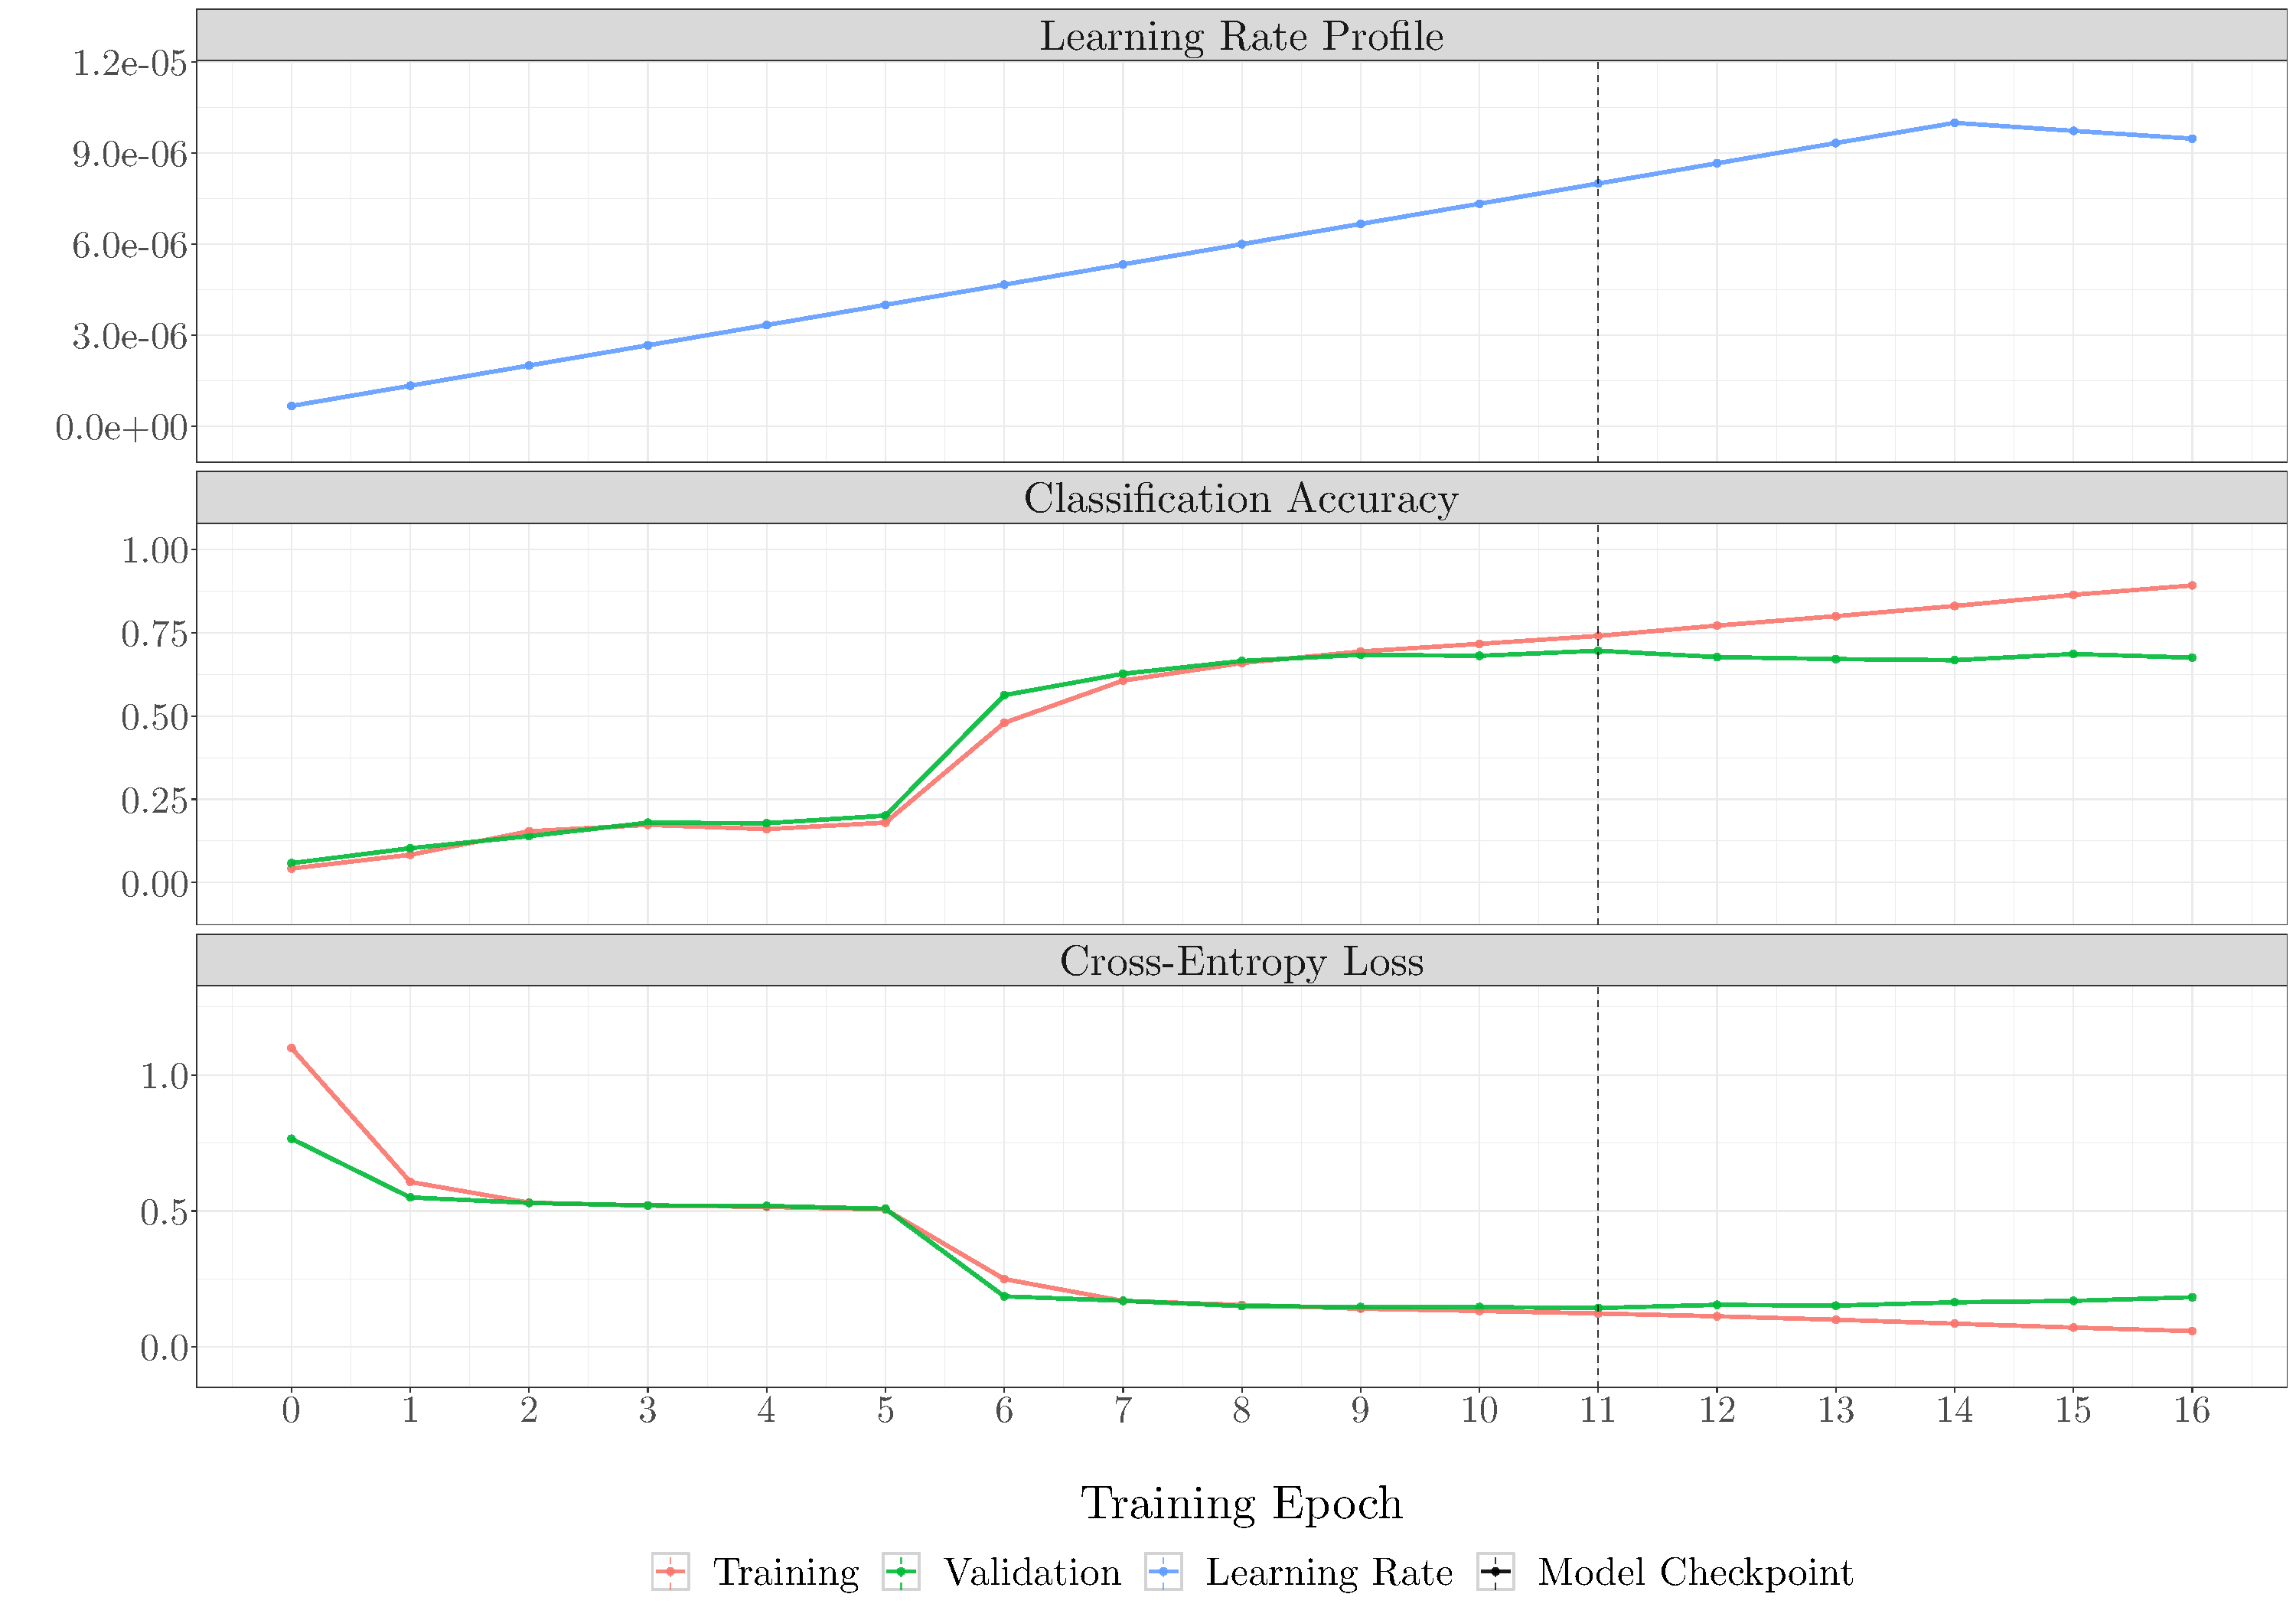
\includegraphics[trim={1.0cm 0cm 0cm 0cm},clip,width=\textwidth]{img/model_training_evolution.pdf}
    \caption{TD$\_$Dense model performance summary statistics by training epochs; black vertical line demarcates the 12th training epoch where validation cross-entropy loss was minimized}
    \label{model_performance}
\end{figure}

\subsubsection{Prediction on UNSC}

After identifying the best model as the TD$\_$Dense model, we then used this model to predict token-level argumentation labels of the preprocessed (pruned) UNSC corpus. Figure \ref{unsc_pred} shows the token distribution of the predictions of our best classifier on the UNSC corpus. Similar to the token distributions in the USED corpus as shown in Figure \ref{used_distribution_combined}, we observe that the proportions of claim and premise tokens, as well as argumentative speeches, increase as the speech sequence lengths increase. However, unlike the USED corpus' balanced token/speech distributions in Figure \ref{used_distribution_combined}; our fine-tuned model's predictions appear to show a strong skew towards N tokens and non-argumentative speeches.

There could be many reasons for this; one of which could be a bias towards more informal argumentation structures in the USED corpus which might conflict with the formalized argumentation structures in the UNSC corpus. In section \ref{manual_semantic}, we will perform some manual semantic analyses of positive and negative UNSC predictions to sample, albeit in an extremely limited manner, performance on the UNSC corpus. 

\begin{figure}[t!]
    \centering
    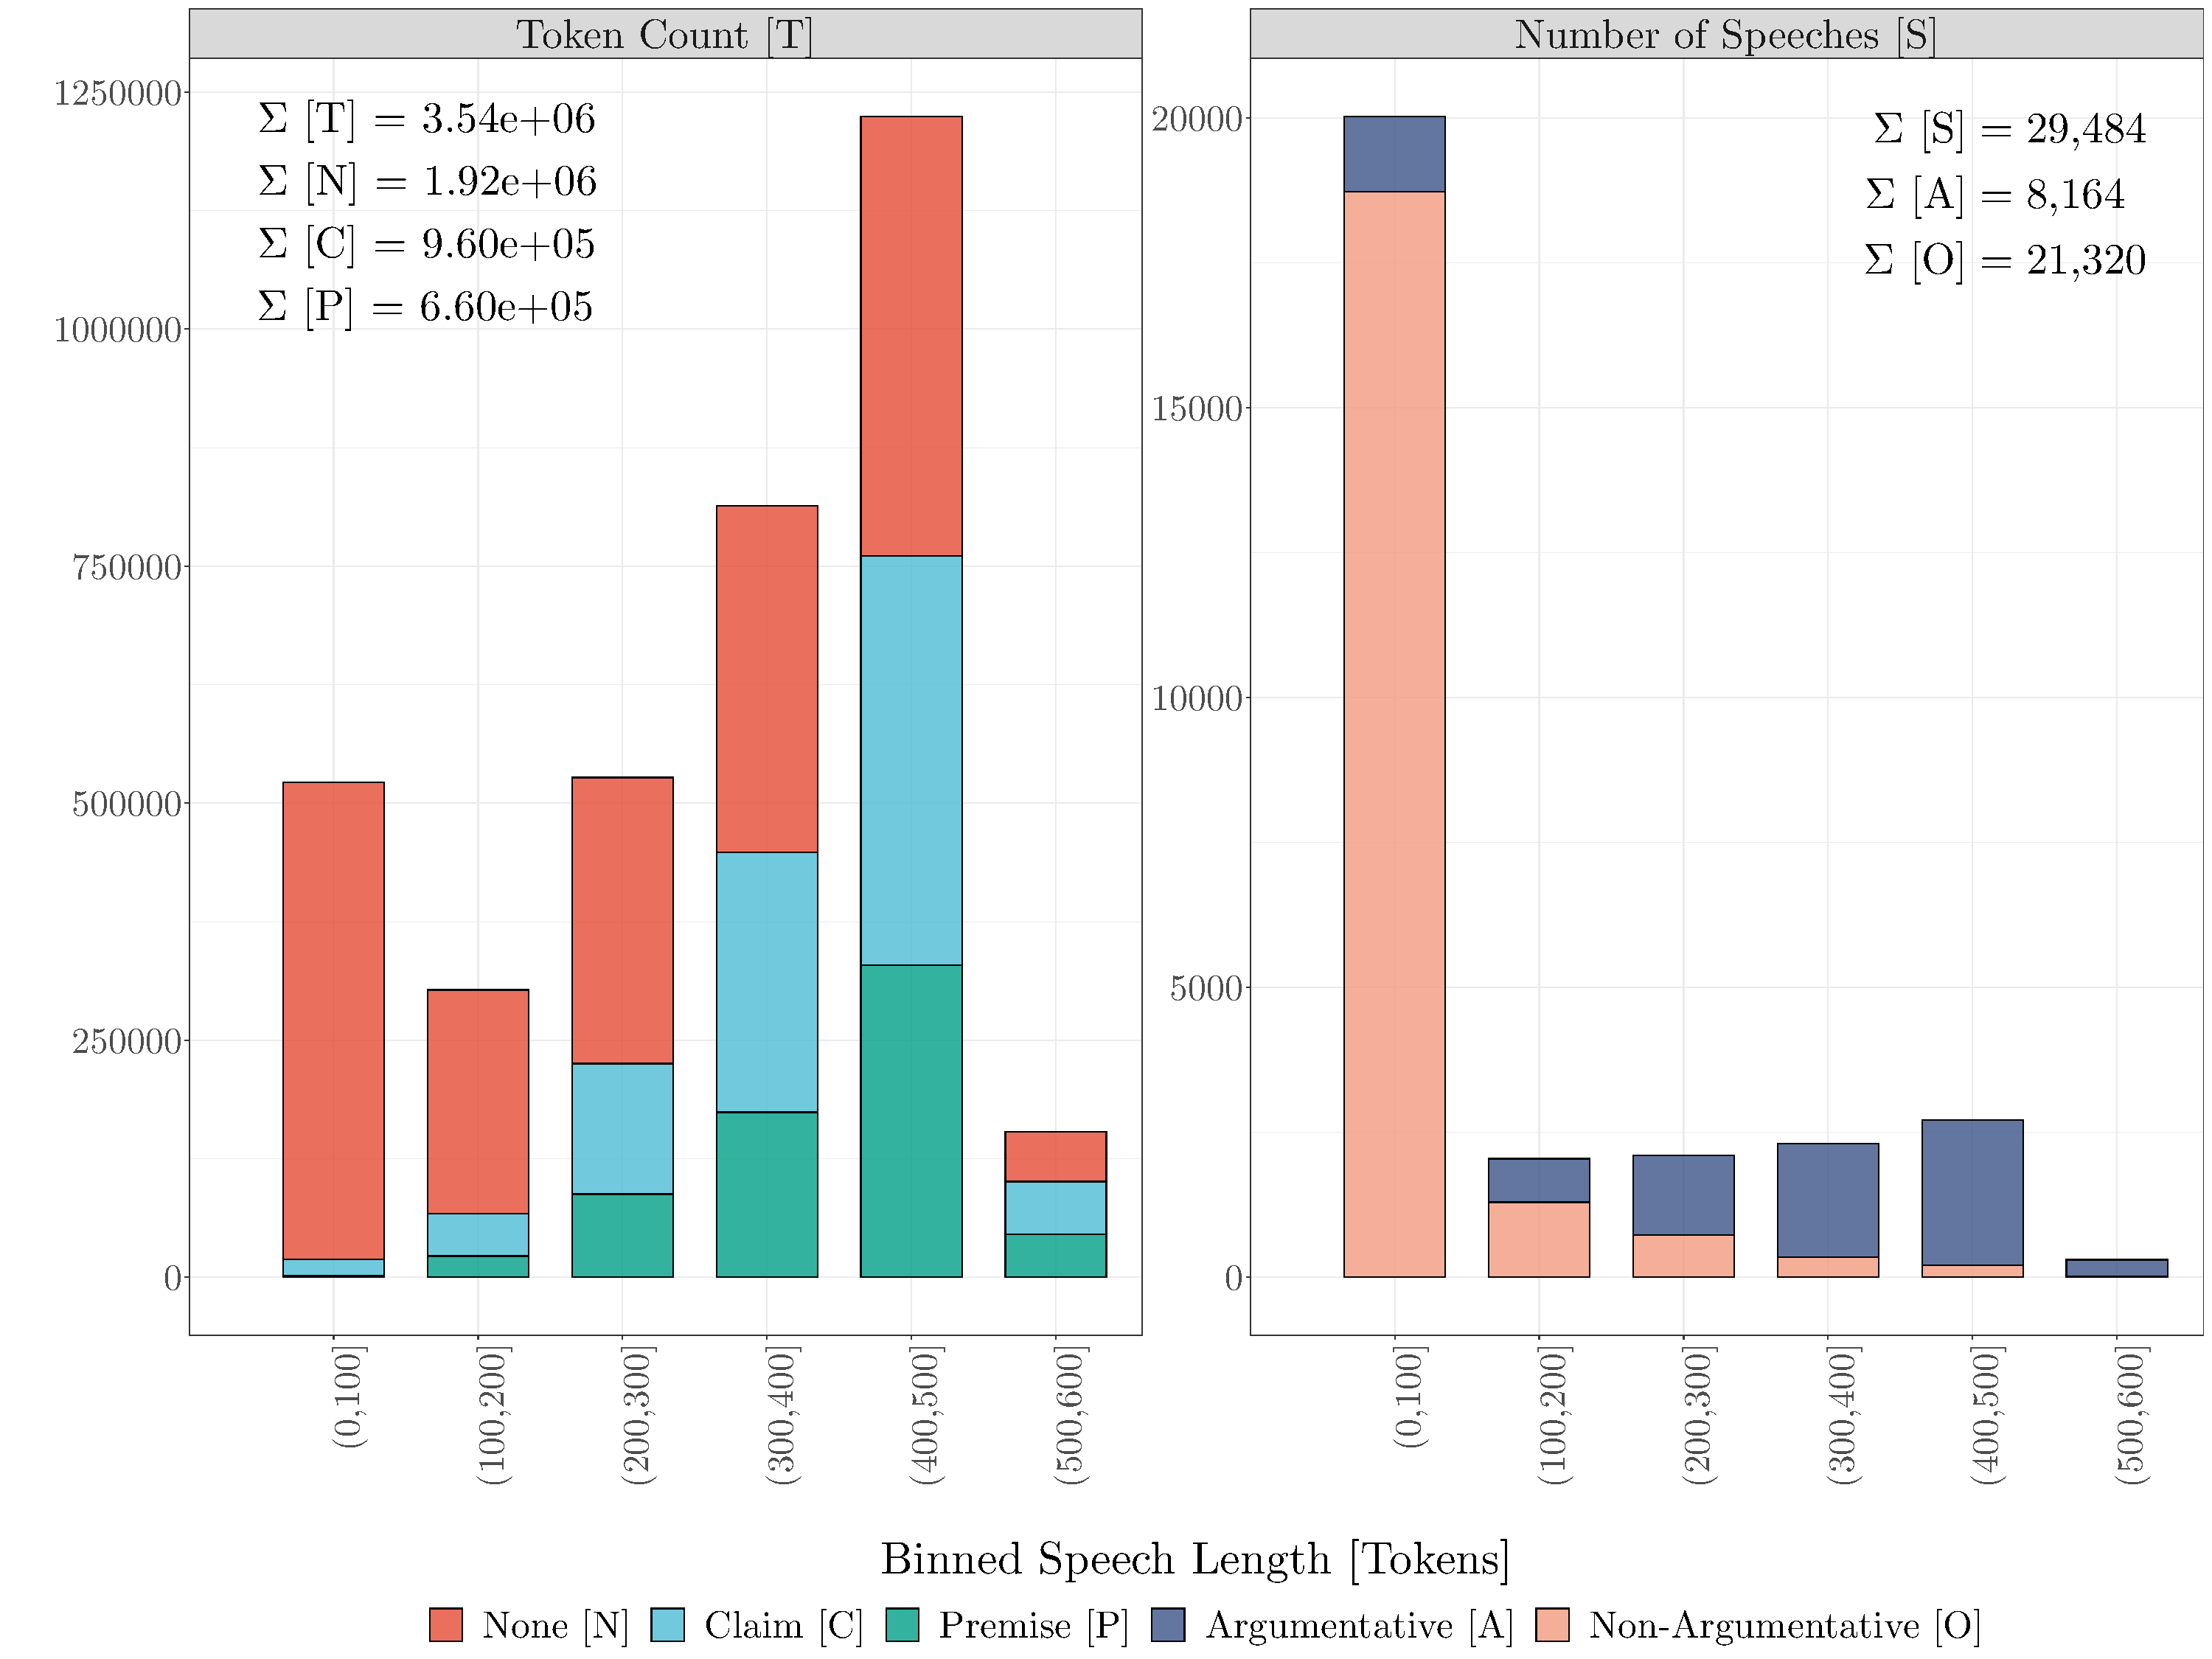
\includegraphics[trim={1.0cm 0cm 0cm
    0cm},clip,width=\textwidth]{img/token_dist_pred_UNSC_length.pdf}
    \caption{Token type predictions from TD$\_$Dense classifier on pruned UNSC corpus; non-argumentative (O) speeches have zero C and P tokens while argumentative (A) speeches contain at least one of either}
    \label{unsc_pred}
\end{figure}